\chapter{\textsl{Prolog}} 
Im diesem Kapitel wollen wir uns mit dem logischen Programmieren und der
Sprache \textsl{Prolog} besch\"{a}ftigen.  Der Name \textsl{Prolog} steht f\"{u}r 
``\emph{\underline{pro}gramming in \underline{log}ic}''.
Die Grundidee des logischen Programmieren 
kann wie folgt dargestellt werden:
\begin{enumerate}
\item Der Software-Entwickler erstellt eine \emph{Wissensbasis}.
      Diese enth\"{a}lt Informationen in Form von \emph{Fakten} und \emph{Regeln}.
\item Ein automatischer Beweiser (eine sogenannte \emph{Inferenz-Maschine})
      erschlie\3t aus diesen Fakten und Regeln
      Informationen und beantwortet so Anfragen.
\end{enumerate}
Das Besondere an dieser Art der Probleml\"{o}sung besteht darin, dass es nicht mehr notwendig
ist, einen Algorithmus zu entwickeln, der ein bestimmtes Problem l\"{o}st.  Statt dessen
wird das Problem durch logische Formeln beschrieben.  Zur L\"{o}sung des Problems
wird dann ein automatischen Beweiser eingesetzt, der die gesuchte L\"{o}sung berechnet.
Diese Vorgehensweise folgt dem Paradigma des \emph{deklarativen Programmierens}.
In der Praxis funktioniert der deklarative Ansatz nur bei einfachen Beispielen.  Um mit
Hilfe von \textsl{Prolog} auch komplexere Aufgaben l\"{o}sen zu k\"{o}nnen, ist es unumg\"{a}nglich, die
Funktionsweise des eingesetzten automatischen Beweisers zu verstehen.

Wir geben ein einfaches Beispiel, an dem wir das Grundprinzip des deklarativen
Programmierens mit \textsl{Prolog} erl\"{a}utern k\"{o}nnen.  Abbildung \ref{fig:caesar} auf Seite
\pageref{fig:caesar} zeigt ein \textsl{Prolog}-Programm, das aus einer Ansammlung von
\textsl{Fakten} und \textsl{Regeln} besteht:
\begin{enumerate}
\item Ein \emph{Fakt} ist eine atomare Formel.  Die Syntax ist\\[0.2cm]
      \hspace*{1.3cm} $p(t_1,\cdots,t_n).$ \\[0.2cm]
      Dabei ist $p$ ein Pr\"{a}dikats-Zeichen und $t_1, \cdots,t_n$ sind Terme.
      Ist die Menge der Variablen, die in den Termen $t_1,\cdots,t_n$ vorkommen,
      durch $\{x_1,\cdots,x_m\}$ gegeben, so wird der obige Fakt als die 
      logische Formel \\[0.2cm]
      \hspace*{1.3cm} $\forall x_1, \cdots, x_m \colon p(t_1,\cdots,t_n)$ \\[0.2cm]
      interpretiert.  Das Programm in Abbildung \ref{fig:caesar} enth\"{a}lt in den Zeilen
      1 bis 5 Fakten.  Umgangssprachlich k\"{o}nnen wir diese wie folgt lesen:
      \begin{enumerate}
      \item Asterix ist ein Gallier.
      \item Obelix ist ein Gallier.
      \item C\"{a}sar ist ein Kaiser.
      \item C\"{a}sar ist ein R\"{o}mer.
      \end{enumerate}
\item Eine \emph{Regel} ist eine bedingte Aussage.  Die Syntax ist \\[0.2cm]
      \hspace*{1.3cm} 
      $A \;\texttt{:-}\; B_1\texttt{,} \cdots\texttt{,} B_n\texttt{.}$ 
      \\[0.2cm]
      Dabei sind $A$ und $B_1, \cdots, B_n$ atomare Formeln, haben also die Gestalt \\[0.2cm]
      \hspace*{1.3cm} $q(s_1,\cdots,s_k)$,\\[0.2cm]
      wobei $q$ ein Pr\"{a}dikats-Zeichen ist und $s_1, \cdots, s_k$ Terme sind.
      Ist die Menge der Variablen, die in den atomaren Formeln $A,B_1,\cdots,B_n$
      auftreten, durch $\{x_1, \cdots, x_m\}$ gegeben, so wird die obige Regel als die 
      logische Formel       
      \[ \forall x_1, \cdots, x_m : (B_1 \wedge \cdots \wedge B_m \rightarrow A) \]
      interpretiert.  Das Programm aus Abbildung \ref{fig:caesar} enth\"{a}lt in den Zeilen
      7 bis 12 Regeln.  Schreiben wir diese Regeln als pr\"{a}dikatenlogische Formeln,
      so erhalten wir:
      \begin{enumerate}
      \item $\forall x : \bigl(\texttt{gallier}(x) \rightarrow \texttt{stark}(x)\bigr)$


            \textsl{Alle Gallier sind stark.}
      \item $\forall x : \bigl(\texttt{stark}(x) \rightarrow \texttt{maechtig}(x)\bigr)$

            \textsl{Wer stark ist, ist m\"{a}chtig.}
      \item $\forall x : \bigl(\texttt{kaiser}(x) \wedge \texttt{roemer}(x) \rightarrow \texttt{maechtig}(x)\bigr)$

            \textsl{Wer Kaiser und R\"{o}mer ist, der ist m\"{a}chtig.}
      \item $\forall x : \bigl(\texttt{roemer}(x) \rightarrow \texttt{spinnt}(x)\bigr)$

            \textsl{Wer R\"{o}mer ist, spinnt.}
      \end{enumerate}
\end{enumerate}

\begin{figure}[!h]
  \centering
\begin{Verbatim}[ frame         = lines, 
                  framesep      = 0.3cm, 
                  labelposition = bottomline,
                  numbers       = left,
                  numbersep     = -0.2cm,
                  xleftmargin   = 0.8cm,
                  xrightmargin  = 0.8cm
                ]
    gallier(asterix).
    gallier(obelix).

    kaiser(caesar).
    roemer(caesar).

    stark(X) :- gallier(X).

    maechtig(X) :- stark(X).
    maechtig(X) :- kaiser(X), roemer(X).

    spinnt(X) :- roemer(X).
\end{Verbatim}
\vspace*{-0.3cm}
  \caption{Ein einfaches Prolog-Programm.}
  \label{fig:caesar}
\end{figure}

\noindent
Wir haben in dem Programm in Abbildung \ref{fig:caesar} die Zeile \\[0.2cm]
\hspace*{1.3cm} \texttt{stark(X) :- gallier(X).} \\[0.2cm]
als die Formel \\[0.2cm]
\hspace*{1.3cm} $\forall x \colon \bigl(\texttt{gallier}(x) \rightarrow \texttt{stark}(x)\bigr)$ \\[0.2cm]
interpretiert.  Damit eine solche Interpretation m\"{o}glich ist, muss klar sein,
dass in der obigen Regel der String ``\texttt{X}'' eine Variable bezeichnet,
w\"{a}hrend die Strings ``\texttt{stark}'' und ``\texttt{gallier}'' Pr\"{a}dikats-Zeichen sind. 
Prolog hat sehr einfache syntaktische Regeln um Variablen von Pr\"{a}dikats- und Funktions-Zeichen
unterscheiden zu k\"{o}nnen:
\begin{enumerate}
\item Wenn ein String mit einem gro\3en Buchstaben oder aber mit dem Unterstrich
      ``\texttt{\_}'' beginnt und nur aus Buchstaben, Ziffern und dem Unterstrich
      ``\texttt{\_}'' besteht, dann bezeichnet dieser String eine Variable.
      Die folgenden Strings sind daher Variablen: 
      \\[0.2cm]
      \hspace*{1.3cm} \texttt{X}, \texttt{ABC\_32}, \texttt{\_U}, \texttt{Hugo},
      \texttt{\_1}, \texttt{\_}.
\item Strings, die mit einem kleinen Buchstaben beginnen und nur aus Buchstaben, Ziffern
      und dem Unterstrich ``\texttt{\_}'' bestehen, bezeichnen Pr\"{a}dikats- und Funktions-Zeichen.
      Die folgenden Strings k\"{o}nnen also als Funktions- oder Pr\"{a}dikats-Zeichen
      verwendet werden:
      \\[0.2cm]
      \hspace*{1.3cm}      
      \texttt{asterix}, \texttt{a1}, \texttt{i\_love\_prolog}, \texttt{x}.
\item Die Strings \\[0.2cm]
      \hspace*{1.3cm} 
      ``\texttt{+}'',
      ``\texttt{-}'',
      ``\texttt{*}'',
      ``\texttt{/}'',
      ``\texttt{.}'' \\[0.2cm]
      bezeichnen Funktions-Zeichen.  Bis auf das Funktions-Zeichen ``\texttt{.}''
      k\"{o}nnen diese Funktions-Zeichen auch, wie in der Mathematik \"{u}blich,
      als Infix-Operatoren geschrieben werden.  Das Funktions-Zeichen ``\texttt{.}''
      bezeichnen wir als \emph{Dot-Operator}.  Dieser Operator wird zur Konstruktion von
      Listen benutzt.  Die Details werden wir sp\"{a}ter diskutieren.
\item Die Strings \\[0.2cm]
      \hspace*{1.3cm} 
      ``\texttt{<}'',
      ``\texttt{>}'',
      ``\texttt{=}'',
      ``\texttt{=<}'',
      ``\texttt{>=}'',  
      ``\texttt{$\backslash$=}'', 
      ``\texttt{==}'',
      ``\texttt{$\backslash$==}''.
      \\[0.2cm]
      bezeichnen Pr\"{a}dikats-Zeichen. Auch f\"{u}r diese Pr\"{a}dikats-Zeichen ist eine
      Infix-Schreibweise zul\"{a}ssig.
      
      Gegen\"{u}ber den Sprachen \texttt{C} und \textsc{SetlX}
      gibt es hier die folgenden Unterschiede, die besonders Anf\"{a}ngern oft
      Probleme bereiten.
      \begin{enumerate}
      \item Bei dem Operator ``\texttt{=<}'' treten die Zeichen ``\texttt{=}''
            und ``\texttt{<}'' nicht in derselben Reihenfolge auf, wie das in den
            Sprachen \texttt{C} oder \textsc{SetlX} der Fall ist, denn dort wird dieser
            Operator als  ``\texttt{<=}'' geschrieben. 
      \item Der Operator ``\texttt{==}'' testet, ob die beiden Argumente gleich sind,
            w\"{a}hrend der Operator ``\texttt{$\backslash$==}'' testet, ob die beiden Werte
            ungleich sind.  In \texttt{C} und \textsc{SetlX} hat der entsprechende Operator
            die Form ``\texttt{!=}''.
      \item Der Operator ``\texttt{=}'' ist der Unifikations-Operator.
            Bei einem Aufruf der Form 
            \\[0.2cm]
            \hspace*{1.3cm}
            $s = t$
            \\[0.2cm]
            versucht das \textsl{Prolog}-System die syntaktische Gleichung $s \doteq t$ zu
            l\"{o}sen.\footnote{
              Leider wird dabei im Normalfall der \emph{Occur-Check} \underline{nicht}
              durchgef\"{u}hrt. Durch Eingabe des Befehls
              \\[0.1cm]
              \hspace*{1.3cm}
              \texttt{set\_prolog\_flag(occurs\_check, true).}
              \\[0.1cm]
              k\"{o}nnen Sie aber erzwingen, dass bei jeder Unifikation ein Occur-Check
              durchgef\"{u}hrt wird.
            }
            Falls dies erfolgreich ist, werden die Variablen, die in den 
            Termen $s$ und $t$ vorkommen, \emph{instantiiert}.  Was dabei im Detail 
            passiert, werden wir sp\"{a}ter sehen.

            Der Operator ``{$\backslash$=}'' bezeichnet die Negation des Unifikations-Operators.
     \end{enumerate}
      
\item Zahlen bezeichnen 0-stellige Funktions-Zeichen. In \textsl{Prolog} k\"{o}nnen Sie sowohl
      ganze Zahlen als auch Flie\3komma-Zahlen benutzen.  Die Syntax f\"{u}r Zahlen ist \"{a}hnlich
      wie in \texttt{C}, die folgenden Strings stellen also Zahlen dar:
      \\[0.2cm]
      \hspace*{1.3cm}      
      \texttt{12}, \texttt{-3}, \texttt{2.5}, \texttt{2.3e-5}.
\end{enumerate}

Nachdem wir jetzt Syntax und Semantik des Programms in Abbildung \ref{fig:caesar}
erl\"{a}utert haben, zeigen wir nun, wie \textsl{Prolog} sogenannte \emph{Anfragen}
beantwortet. Wir nehmen an, dass das Programm in einer Datei mit dem Namen
``\texttt{gallier.pl}'' abgespeichert ist.  Wir wollen herausfinden, ob es jemanden gibt,
der einerseits m\"{a}chtig ist und der andererseits spinnt.  Logisch wird dies durch die
folgende Formel ausgedr\"{u}ckt: \\[0.2cm]
\hspace*{1.3cm} $\exists x \colon \bigl(\texttt{maechtig}(x) \wedge \texttt{spinnt}(x)\bigr)$. \\[0.2cm]
Als \textsl{Prolog}-Anfrage k\"{o}nnen wir den Sachverhalt wie folgt formulieren: \\[0.2cm]
\hspace*{1.3cm} \texttt{maechtig(X), spinnt(X).} \\[0.2cm]
Um diese Anfrage auswerten zu k\"{o}nnen, starten wir das \textsl{SWI-Prolog}-System\footnote{
Sie finden dieses Prolog-System im Netz unter \href{http://www.swi-prolog.org}{\texttt{www.swi-prolog.org}}.}
in einer Shell mit dem Kommando: \\[0.2cm]
\hspace*{1.3cm} \texttt{swipl}\\[0.2cm]
Wenn das \textsl{Prolog}-System installiert ist, begr\"{u}\3t uns das System wie folgt:
\begin{verbatim}
    Welcome to SWI-Prolog (Multi-threaded, 64 bits, Version 6.6.1-DIRTY)
    Copyright (c) 1990-2013 University of Amsterdam, VU Amsterdam
    SWI-Prolog comes with ABSOLUTELY NO WARRANTY. This is free software,
    and you are welcome to redistribute it under certain conditions.
    Please visit http://www.swi-prolog.org for details.
    
    For help, use ?- help(Topic). or ?- apropos(Word).
    
    ?- 
\end{verbatim}
Die Zeichenfolge ``\texttt{?-}'' ist der \textsl{Prolog}-Prompt.  Hier geben wir  \\[0.2cm]
\hspace*{1.3cm} \texttt{consult(gallier).} \\[0.2cm]
ein (und zwar mit dem Punkt) und dr\"{u}cken \textsl{Return}. Damit fordern wir das System auf, die
Fakten und Regeln aus der Datei ``\texttt{gallier.pl}'' zu laden.  Als Ergebnis erhalten
wir die Meldung
\begin{verbatim}
    ?- consult(gallier).
    % gallier compiled 0.00 sec, 1,676 bytes
    
    Yes
    ?- 
\end{verbatim}
Das Programm wurde erfolgreich geladen und \"{u}bersetzt.  Wir geben nun unsere Anfrage ein

\begin{verbatim}
    ?- maechtig(X), spinnt(X).
\end{verbatim}
und erhalten als Antwort:
\begin{verbatim}
    X = caesar.
\end{verbatim}
Da diese Antwort mit einem Punkt ``\texttt{.}'' beendet wird, k\"{o}nnen wir folgern, dass es keine
weiteren m\"{o}glichen Antworten gibt, die logisch aus den Fakten und Regeln folgen.  W\"{u}rde es noch
weitere Antworten geben, so h\"{a}tte die Antwort nur die Form 
\begin{verbatim}
    X = caesar
\end{verbatim}
gehabt.  In diesem Fall h\"{a}tten wir zwei M\"{o}glichkeiten gehabt:
\begin{enumerate}
\item Wenn wir mit dieser Antwort zufrieden sind, dr\"{u}cken wir \textsl{Return} und erhalten einen
      neuen Prompt.
\item Wenn wir statt dessen nach weiteren Personen suchen wollen, die einerseits
      m\"{a}chtig sind und andererseits spinnen, dann geben wir das Zeichen ``\texttt{;}'' ein.
      In diesem Fall h\"{a}tte das System versucht, weitere m\"{o}gliche Antworten zu finden.
\end{enumerate} 
Wenn wir das \textsl{Prolog}-System wieder verlassen wollen, dann geben wir den Befehl
``\texttt{halt}.'' ein.

\section{Wie arbeitet \textsl{Prolog}?}
Das Konzept des logischen Programmierens sieht vor, dass der Benutzer eine Datenbank mit
Fakten und Regeln erstellt, die das Problem vollst\"{a}ndig beschreiben.  Anschlie\3end
beantwortet dann das \textsl{Prolog}-System m\"{o}gliche Anfragen mit Hilfe einer
Inferenz-Maschine.  Um nicht-triviale \textsl{Prolog}-Programme erstellen zu k\"{o}nnen, ist es
notwendig zu verstehen, wie das \textsl{Prolog}-System Anfragen beantwortet.
Um diesen Algorithmus leichter darstellen zu k\"{o}nnen, vereinbaren wir folgendes:
Ist ein Fakt der Form \\[0.2cm]
\hspace*{1.3cm} $A$.
\\[0.2cm]
gegeben, so formen wir dies zu der Regel \\[0.2cm]
\hspace*{1.3cm} $A \;\texttt{:-}\; \texttt{true}.$ \\[0.2cm]
um.  Au\3erdem bezeichnen wir bei einer Klausel \\[0.2cm]
\hspace*{1.3cm} $A \;\texttt{:-}\; B_1, \cdots, B_n$. \\[0.2cm]
die atomare Formel $A$ als den \emph{Kopf} und die Konjunktion $B_1, \cdots, B_n$
als den \emph{Rumpf} der Klausel.
\vspace*{0.2cm}

Wir beschreiben nun den Algorithmus, mit dem das \textsl{Prolog}-System Anfragen
beantwortet. 

\noindent
\begin{enumerate}
\item \textbf{Gegeben}
      \begin{enumerate}
      \item Anfrage: \quad  $G = Q_1, \cdots, Q_n$

            Hier sind $Q_1, \cdots, Q_n$ atomare Formeln.
      \item \textsl{Prolog}-Programm: \quad $P$
            \vspace*{0.1cm}
        
            Da die Reihenfolge der Klauseln f\"{u}r das Folgende relevant ist, fassen wir das
            \textsl{Prolog}-Programm $P$ als Liste von Regeln auf.
      \end{enumerate}
\item \textbf{Gesucht}: Eine Substitution $\sigma$, so dass die Instanz $G\sigma$ aus den
      Regeln des Programms $P$ folgt: 
      \[ \models \forall (P) \rightarrow \forall(G\sigma). \]
      Hier bezeichnet $\forall(P)$ den Allabschluss der Konjunktion aller Klauseln aus $P$
      und $\forall(G\sigma)$ bezeichnet entsprechend den Allabschluss von $G\sigma$.
\end{enumerate}
Der Algorithmus selbst arbeitet wie folgt:
\begin{enumerate}
\item Suche (der Reihe nach) in dem Programm $P$ alle Regeln        
      \[ A \;\texttt{:-}\; B_1,\cdots,B_m. \] 
      f\"{u}r die der Unifikator $\mu = \texttt{mgu}(Q_1,A)$ existiert.
\item Gibt es mehrere solche Regeln, so
      \begin{enumerate}
      \item w\"{a}hlen wir die erste Regel aus, wobei wir uns an der Reihenfolge orientieren,
            in der die Regeln in dem Programm $P$ auftreten.
      \item Au\3erdem setzen wir an dieser Stelle einen Auswahl-Punkt (\emph{Choice-Point}),
            um sp\"{a}ter hier eine andere Regel w\"{a}hlen zu k\"{o}nnen, falls dies notwendig werden
            sollte.
      \end{enumerate}
\item Wir setzen $G := G\mu$, wobei $\mu$ der oben berechnete Unifikator ist.
\item Nun   bilden wir die  Anfrage \\[0.2cm]
      \hspace*{1.3cm} $B_1\mu, \cdots, B_m\mu, Q_2\mu, \cdots, Q_n\mu$. \\[0.2cm]
      Jetzt k\"{o}nnen zwei F\"{a}lle auftreten: 
      \begin{enumerate}
      \item $m + n = 0$: Dann ist die Beantwortung der Anfrage erfolgreich und wir geben
            als Antwort $G\mu$ zur\"{u}ck.
      \item Sonst beantworten wir rekursiv die Anfrage $B_1\mu, \cdots, B_m\mu, Q_2\mu, \cdots, Q_n\mu$            . 
        
            Falls die rekursive Beantwortung unter Punkt 4 erfolglos war,
            gehen wir zum letzten Auswahl-Punkt  zur\"{u}ck.  Gleichzeitig werden alle Zuweisungen
            $G := G\mu$, die wir seit diesem Auswahl-Punkt durchgef\"{u}hrt haben, wieder r\"{u}ckg\"{a}ngig
            gemacht.  Anschlie\3end versuchen wir, mit der n\"{a}chsten m\"{o}glichen Regel
            die Anfrage zu beantworten.
      \end{enumerate}
\end{enumerate}
Um den Algorithmus besser zu verstehen, beobachten wir die Abarbeitung der Anfrage \\[0.2cm]
\hspace*{1.3cm} \texttt{maechtig(X), spinnt(X).} \\[0.2cm]
im Debugger des \textsl{Prolog}-Systems.  Wir geben dazu nach dem Laden des
Programms ``\texttt{gallier.pl}'' das Kommando \texttt{guitracer} ein.
\begin{verbatim}
?- guitracer.
\end{verbatim}
Wir erhalten die Antwort:
\begin{verbatim}
% The graphical front-end will be used for subsequent tracing

Yes
?- 
\end{verbatim}
Jetzt starten wir die urspr\"{u}ngliche Anfrage noch einmal, setzen aber das Kommando
\texttt{trace} vor unsere Anfrage:
\begin{verbatim}
    ?- trace, maechtig(X), spinnt(X).
\end{verbatim}
Als Ergebnis wird ein Fenster ge\"{o}ffnet, das Sie in Abbildung \ref{fig:debugger} auf Seite
\pageref{fig:debugger} sehen.  Unter dem Men\"{u} sehen Sie hier eine Werkzeugleiste.
Die einzelnen Symbole haben dabei die folgende Bedeutung:
\begin{enumerate}
\item Die Schaltfl\"{a}che \raisebox{-0.2cm}{
\epsfig{file=Figures/down.eps}}
      dient dazu, einzelne Unifikationen anzuzeigen.  Mit dieser Schaltfl\"{a}che
      k\"{o}nnen wir die meisten Details der Abarbeitung beobachten.

      Alternativ hat die Taste ``\texttt{i}'' dieselbe Funktion.
\item Die Schaltfl\"{a}che \raisebox{-0.2cm}{
\epsfig{file=Figures/step.eps}}
      dient dazu, einen einzelnen Schritt bei der Abarbeitung einer Anfrage
      durchzuf\"{u}hren.

      Alternativ hat die Leertaste dieselbe Funktion.
\item Die Schaltfl\"{a}che \raisebox{-0.2cm}{
\epsfig{file=Figures/skip.eps}}
      dient dazu, die n\"{a}chste atomare Anfrage in einem Schritt durchzuf\"{u}hren.
      Dr\"{u}cken wir diese Schaltfl\"{a}che unmittelbar, nachdem wir das Ziel \\[0.2cm]
      \hspace*{1.3cm} \texttt{maechtig(X), roemer(X).} \\[0.2cm]
      eingegeben haben, so w\"{u}rde der Debugger die Anfrage
      \texttt{maechtig(X)} in einem Schritt beantworten.  Dabei w\"{u}rde dann die Variable
      \texttt{X} an die Konstante \texttt{asterix} gebunden.

      Alternativ hat die Taste ``\texttt{s}'' (\emph{skip}) dieselbe Funktion.
\item Die Schaltfl\"{a}che \raisebox{-0.2cm}{
\epsfig{file=Figures/finish.eps}} dient dazu,
      die Prozedur, in deren Abarbeitung wir uns befinden, ohne Unterbrechung zu Ende
      abarbeiten zu lassen.  Versuchen wir beispielsweise die atomare Anfrage ``\texttt{maechtig(X)}''
      mit der Regel \\[0.2cm]
      \hspace*{1.3cm} \texttt{maechtig(X) :- kaiser(X), roemer(X).} \\[0.2cm]
      abzuarbeiten und m\"{u}ssen nun die Anfrage ``\texttt{kaiser(X), roemer(X).}''
      beantworten, so w\"{u}rden wir durch Bet\"{a}tigung dieser Schaltfl\"{a}che sofort die Antwort
      ``\texttt{X = caesar}'' f\"{u}r diese Anfrage erhalten.

      Alternative hat die Taste ``\texttt{f}'' (\emph{finish}) dieselbe Funktion.
\item Die Schaltfl\"{a}che \raisebox{-0.2cm}{
\epsfig{file=Figures/redo.eps}} 
      dient dazu, eine bereits beantwortete Anfrage noch einmal zu beantworten.
      Dies kann sinnvoll sein, wenn man beim Tracen einer Anfrage nicht aufgepasst hat
      und noch einmal sehen m\"{o}chte, wie das \textsl{Prolog}-System zu seiner Antwort
      gekommen ist.
      
      Alternative hat die Taste ``\texttt{r}'' (\emph{retry}) dieselbe Funktion.
\item Die Schaltfl\"{a}che \raisebox{-0.2cm}{
\epsfig{file=Figures/nodebug.eps}}
      beantwortet die gestellte Anfrage ohne weitere Unterbrechung.

      Alternative hat die Taste ``\texttt{n}'' (\emph{nodebug}) dieselbe Funktion.

      Von den weiteren Schaltfl\"{a}chen sind f\"{u}rs erste nur noch zwei interessant.
\item Die Schaltfl\"{a}che \raisebox{-0.2cm}{
\epsfig{file=Figures/continue.eps}}
       l\"{a}sst das Programm bis zum n\"{a}chsten Haltepunkt laufen.

      Alternative hat die Taste ``\texttt{l}'' (\emph{continue}) dieselbe Funktion.
\item Die Schaltfl\"{a}che \raisebox{-0.2cm}{
\epsfig{file=Figures/break.eps}} 
      setzt einen Haltepunkt.  Dazu muss vorher der Cursor an die Stelle gebracht
      werden, an der ein Haltepunkt gesetzt werden soll.

      Alternative hat die Taste ``\texttt{!}''  dieselbe Funktion.
\end{enumerate}

\begin{figure}[!h]
  \centering
  \framebox{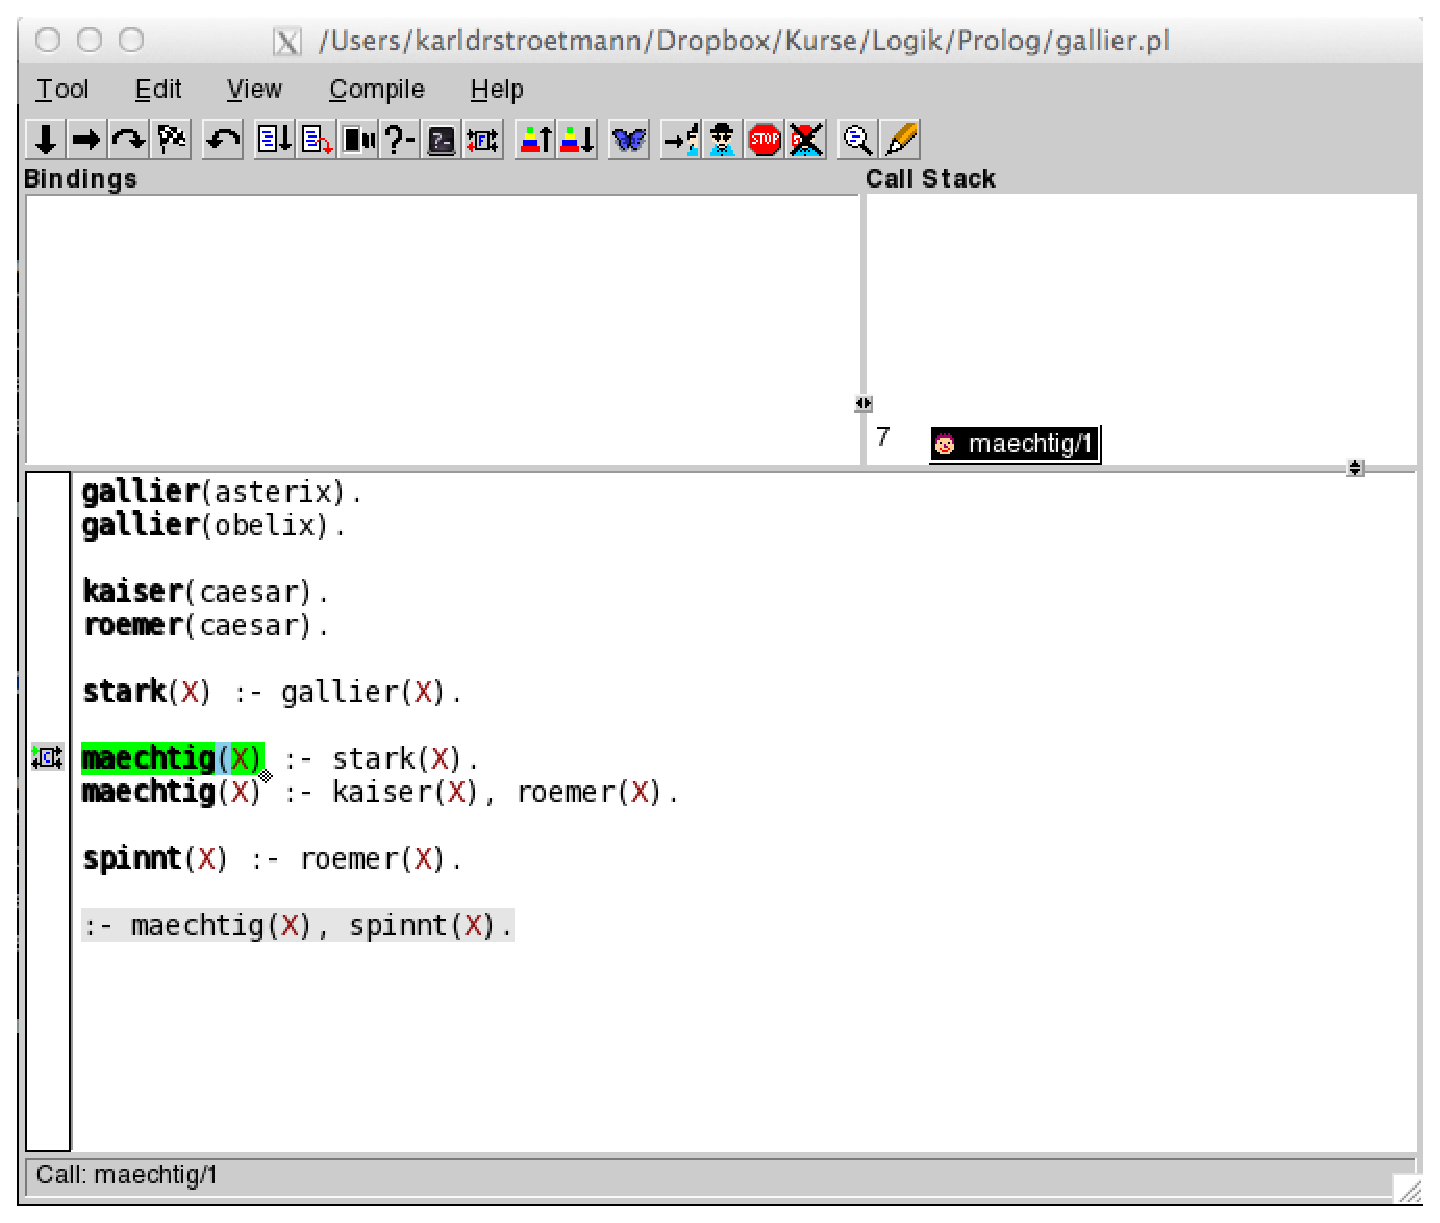
\epsfig{file=Figures/debug.eps,scale=0.7}} 
  \caption{Der Debugger des \textsl{SWI-Prolog}-Systems.}
  \label{fig:debugger}
\end{figure}

Wir zeigen, wie das Ziel \texttt{maechtig(X), spinnt(X)} 
vom \textsl{Prolog}-System beantwortet wird.  
\begin{enumerate}
\item Zun\"{a}chst wird versucht, die Anfrage ``\texttt{maechtig(X)}'' zu l\"{o}sen.
      Die erste Regel, die das Pr\"{a}dikat \texttt{maechtig/1} definiert,
      ist \\[0.2cm]
      \hspace*{1.3cm} \texttt{maechtig(X) :- stark(X).}\\[0.2cm]
      Daher wird die Anfrage ``\texttt{maechtig(X)}'' reduziert zu der Anfrage 
      ``\texttt{stark(X)}''.  Die aktuelle vollst\"{a}ndige Anfrage lautet nun \\[0.2cm]
      \hspace*{1.3cm} \texttt{stark(X), spinnt(X)}. \\[0.2cm]
      Da es noch eine zweite Regel gibt, die das Pr\"{a}dikat \texttt{maechtig/1} definiert,
      setzen wir an dieser Stelle einen Auswahl-Punkt (\emph{Choice-Point}).  Falls also die 
      Beantwortung der Anfrage ``\texttt{stark(X), spinnt(X)}'' sp\"{a}ter scheitert,
      k\"{o}nnen wir es mit der zweiten Regel noch einmal versuchen.
\item Jetzt wird versucht, die Anfrage ``\texttt{stark(X)}'' zu l\"{o}sen.
      Die erste und einzige Regel, die das Pr\"{a}dikat \texttt{stark/1} definiert, ist 
      \\[0.2cm]
      \hspace*{1.3cm} \texttt{stark(X) :- gallier(X).} \\[0.2cm]
      Nach der Unifikation des Kopfes dieser Regel mit der Anfrage ``\texttt{stark(X)}''
      lautet die aktuelle Anfrage \\[0.2cm]
      \hspace*{1.3cm} 
      \texttt{gallier(X), spinnt(X).}
\item Die erste Regel, die das Pr\"{a}dikat \texttt{gallier/1} definiert und deren Kopf
      mit der Anfrage ``\texttt{gallier(X)}'' unifiziert werden kann, ist der Fakt \\[0.2cm]
      \hspace*{1.3cm} \texttt{gallier(asterix).} \\[0.2cm]
      Bei der Unifikation mit diesem Fakt wird die Variable \texttt{X} an die Konstante
      \texttt{asterix} gebunden.  Damit lautet jetzt die aktuelle Anfrage \\[0.2cm]
      \hspace*{1.3cm} 
      \texttt{spinnt(asterix).} \\[0.2cm]
      Da es noch eine zweite Regel gibt, die das Pr\"{a}dikat \texttt{gallier/1} definiert,
      setzen wir an dieser Stelle einen Auswahl-Punkt.   
\item Die erste und einzige Regel, die das Pr\"{a}dikat \texttt{spinnt/1} definiert,
      lautet \\[0.2cm]
      \hspace*{1.3cm} 
      \texttt{spinnt(X) :- roemer(X).} \\[0.2cm]
      Also wird nun die Variable \texttt{X} in dieser Regel mit \texttt{asterix} 
      unifiziert und wir erhalten die Anfrage \\[0.2cm]
      \hspace*{1.3cm} 
      \texttt{roemer(asterix).}
\item Die einzige Regel, die das Pr\"{a}dikat \texttt{roemer/1} definiert, ist \\[0.2cm]
      \hspace*{1.3cm} 
      \texttt{roemer(caesar).} \\[0.2cm]
      Diese Regel l\"{a}sst sich nicht mit der Anfrage ``\texttt{roemer(asterix)}'' unifizieren.
      Also scheitert diese Anfrage.
\item Wir schauen nun, wann wir das letzte mal einen Auswahl-Punkt gesetzt haben.
      Wir stellen fest, dass wir unter Punkt 3 bei der Beantwortung der Anfrage
      \texttt{gallier(X)} das letzte Mal einen Auswahl-Punkt gesetzt haben.
      Also gehen wir nun zu Punkt 3 zur\"{u}ck und versuchen wieder, die Anfrage
      \\[0.2cm]
      \hspace*{1.3cm} 
      \texttt{gallier(X), spinnt(X)} \\[0.2cm]
      zu l\"{o}sen.  Diesmal w\"{a}hlen wir jedoch den Fakt \\[0.2cm]
      \hspace*{1.3cm} \texttt{gallier(obelix).}  \\[0.2cm]
      Wir erhalten dann die neue Anfrage \\[0.2cm]
      \hspace*{1.3cm} \texttt{spinnt(obelix).}
\item Die erste und einzige Regel, die das Pr\"{a}dikat \texttt{spinnt/1} definiert,
      lautet \\[0.2cm]
      \hspace*{1.3cm} 
      \texttt{spinnt(X) :- roemer(X).} \\[0.2cm]
      Also wird die Variable \texttt{X} in dieser Regel mit \texttt{obelix} 
      unifiziert und wir erhalten die Anfrage \\[0.2cm]
      \hspace*{1.3cm} 
      \texttt{roemer(obelix).}
\item Die einzige Regel, die das Pr\"{a}dikat \texttt{roemer/1} definiert, ist \\[0.2cm]
      \hspace*{1.3cm} 
      \texttt{roemer(caesar).} \\[0.2cm]
      Diese Regel l\"{a}sst sich nicht mit der Anfrage ``\texttt{roemer(asterix)}'' unifizieren.
      Also scheitert diese Anfrage.
\item Wir schauen wieder, wann das letzte Mal ein Auswahl-Punkt gesetzt wurde.
      Der unter Punkt 3~gesetzte Auswahl-Punkt wurde vollst\"{a}ndig abgearbeitet, dieser
      Auswahl-Punkt kann uns also nicht mehr helfen.
      Aber unter Punkt 1 wurde ebenfalls ein Auswahl-Punkt gesetzt, denn f\"{u}r das Pr\"{a}dikat
      \texttt{maechtig/1} gibt es die weitere Regel \\[0.2cm]
      \hspace*{1.3cm} \texttt{maechtig(X) :- kaiser(X), roemer(X)}. \\[0.2cm]
      Wenden wir diese Regel an, so erhalten wir die Anfrage \\[0.2cm]
      \hspace*{1.3cm} 
      \texttt{kaiser(X), roemer(X), spinnt(X).}
\item F\"{u}r das Pr\"{a}dikat \texttt{kaiser/1} enth\"{a}lt unsere Datenbank genau einen Fakt:\\[0.2cm]
      \hspace*{1.3cm} \texttt{kaiser(caesar).}  \\[0.2cm]
      Benutzen wir diesen Fakt zur Reduktion unserer Anfrage, so  lautet die neue Anfrage \\[0.2cm]
      \hspace*{1.3cm} 
      \texttt{roemer(caesar), spinnt(caesar).}
\item F\"{u}r das Pr\"{a}dikat \texttt{roemer/1} enth\"{a}lt unsere Datenbank genau einen Fakt:\\[0.2cm]
      \hspace*{1.3cm} \texttt{roemer(caesar).}  \\[0.2cm]
      Benutzen wir diesen Fakt zur Reduktion unserer Anfrage, so  lautet die neue Anfrage \\[0.2cm]
      \hspace*{1.3cm} 
      \texttt{spinnt(caesar).}
\item Die erste und einzige Regel, die das Pr\"{a}dikat \texttt{spinnt/1} definiert,
      lautet \\[0.2cm]
      \hspace*{1.3cm} 
      \texttt{spinnt(X) :- roemer(X).} \\[0.2cm]
      Also wird die Variable \texttt{X} in dieser Regel mit \texttt{caesar} 
      unifiziert und wir erhalten die Anfrage \\[0.2cm]
      \hspace*{1.3cm} 
      \texttt{roemer(caesar).}
\item F\"{u}r das Pr\"{a}dikat \texttt{roemer/1} enth\"{a}lt unsere Datenbank genau einen Fakt:\\[0.2cm]
      \hspace*{1.3cm} \texttt{roemer(caesar).}  \\[0.2cm]
      Benutzen wir diesen Fakt zur Reduktion unserer Anfrage, so ist die verbleibende
      Anfrage leer.  Damit ist die urspr\"{u}ngliche Anfrage gel\"{o}st.  Die dabei berechnete
      Antwort erhalten wir, wenn wir untersuchen, wie die Variable \texttt{X} unifiziert
      worden ist.  Die Variable \texttt{X} war unter Punkt 10 mit der Konstanten
      \texttt{caesar} unifiziert worden.  Also ist \\[0.2cm]
      \hspace*{1.3cm} \texttt{X = caesar}
      \\[0.2cm]
      die Antwort, die von dem System berechnet wird.
\end{enumerate}
Bei der Beantwortung der Anfrage ``\texttt{maechtig(X), spinnt(X)}'' sind wir einige Male
in Sackgassen hineingelaufen und mussten Instantiierungen der Variable \texttt{X} wieder
zur\"{u}ck nehmen.  Dieser Vorgang wird in der Literatur als \emph{backtracking} bezeichnet.
Er kann mit Hilfe des Debuggers am Bildschirm verfolgt werden.

\subsection{Die Tiefensuche}
Der von Prolog verwendete Such-Algorithmus wird auch als \emph{Tiefensuche} (angels\"{a}chsisch:
\emph{depth first search}) bezeichnet.  Um diesen Ausdruck erl\"{a}utern zu k\"{o}nnen, definieren wir
zun\"{a}chst den Begriff des \emph{Suchbaums}.  Die Knoten eines Suchbaums sind mit Anfrage beschriftet.
Ist der Knoten $u$ des Suchbaums mit der Anfrage
\[ Q_1, \cdots, Q_m \]
beschriftet und gibt es f\"{u}r $i = 1,\cdots,k$ Regeln der Form
\[ A^{(i)} \texttt{:-} B_1^{(i)}, \cdots, B_{n(i)}^{(i)} \]
die auf die Anfrage passen, f\"{u}r die also $\mu_i = \textsl{mgu}(Q_1, A^{(i)})$ existiert, so hat der
Knoten $u$ insgesamt $k$ verschiedene Kinder.  Dabei ist das $i$-te Kind mit der Anfrage
\[  B_1^{(i)}\mu_i, \cdots, B_{n(i)}^{(i)}\mu_i, Q_2\mu_i, \cdots, Q_m\mu_i \]
beschriftet.  Als einfaches Beispiel betrachten wir das in Abbildung \ref{fig:depth.pl} gezeigte
Programm.  Der Suchbaum f\"{u}r die Anfrage
\[ p(X) \]
ist in Abbildung \ref{fig:depth-first.eps} gezeigt.  Den Knoten, der mit der urspr\"{u}nglichen Anfrage
beschriftet ist, bezeichnen wir als die \emph{Wurzel} des Suchbaums.  Die \emph{L\"{o}sungen} zu der
urspr\"{u}nglichen Anfrage finden wir an den \emph{Bl\"{a}ttern} des Baumes: Wir bezeichnen hier die Knoten
als Bl\"{a}tter, die am weitesten unten stehen.  Suchb\"{a}ume stehen also gewisserma\3en auf dem Kopf: Die
Bl\"{a}tter sind unten und die Wurzeln sind oben\footnote{
Daher werden diese Suchb\"{a}ume auch als australische B\"{a}ume bezeichnet.}.

\begin{figure}[!ht]
\centering
\begin{Verbatim}[ frame         = lines, 
                  framesep      = 0.3cm, 
                  labelposition = bottomline,
                  numbers       = left,
                  numbersep     = -0.2cm,
                  xleftmargin   = 0.8cm,
                  xrightmargin  = 0.8cm,
                ]
    p(X) :- q1(X).
    p(X) :- q2(X).
    
    q1(X) :- r1(X). 
    q1(X) :- r2(X). 
    
    q2(X) :- r3(X). 
    q2(X) :- r4(X). 
    
    r1(a).
    r2(b).
    r3(c).
    r4(d).
\end{Verbatim}
\vspace*{-0.3cm}
\caption{Die Tiefensuche in Prolog}
\label{fig:depth.pl}
\end{figure}

\begin{figure}[!ht]
\centering
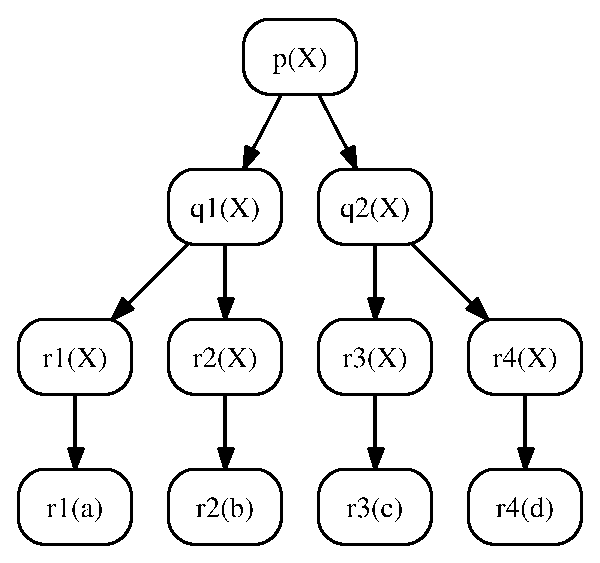
\epsfig{file=depth-first.eps,scale=0.6}

\vspace*{-0.3cm}
\caption{Der Suchbaum f\"{u}r das in Abbildung \ref{fig:depth.pl} gezeigte Programm.}
\label{fig:depth-first.eps}
\end{figure}

Anhand des in Abbildung \ref{fig:depth-first.eps} gezeigten Suchbaums l\"{a}sst sich nun die Tiefensuche
erkl\"{a}ren:  Wenn der Prolog-Interpreter nach einer L\"{o}sung sucht, so w\"{a}hlt er immer den linkesten Ast
und steigt dort so tief wie m\"{o}glich ab.  Dadurch werden die L\"{o}sungen in dem Beispiel in der
Reihenfolge
\[ X = a,\; X = b,\; X = c,\; X = d,\; \]
gefunden.  Die Tiefensuche ist dann problematisch, wenn der linkeste Ast des Suchbaums unendlich
tief ist.  Als Beispiel betrachten wir das  in Abbildung \ref{fig:infinite.pl} gezeigte Prolog-Programm.
Zeichnen wir hier den Suchbaum f\"{u}r die Anfrage
\[ p(X) \]
 so finden wir einen unendlichen Ast, in den der Prolog-Interpreter
absteigt und aus dem er dann mit einem Stack-Overflow wieder zur\"{u}ck kommt.  Vertauschen wir hingegen
die Reihenfolge der Klauseln, so kann das Programm die obige Anfrage beantworten.

\begin{figure}[!ht]
\centering
\begin{Verbatim}[ frame         = lines, 
                  framesep      = 0.3cm, 
                  labelposition = bottomline,
                  numbers       = left,
                  numbersep     = -0.2cm,
                  xleftmargin   = 0.8cm,
                  xrightmargin  = 0.8cm,
                ]
    p(s(X)) :- p(X).
    p(c).
\end{Verbatim}
\vspace*{-0.3cm}
\caption{Eine Endlos-Schleife in \textsl{Prolog}.}
\label{fig:infinite.pl}
\end{figure}

\section{Ein komplexeres Beispiel}
Das obige Beispiel war bewusst einfach gehalten um die Sprache \textsl{Prolog} einzuf\"{u}hren.
Um die M\"{a}chtigkeit des Backtrackings zu demonstrieren, pr\"{a}sentieren wir jetzt ein
komplexeres Beispiel.  Es handelt sich um das folgende R\"{a}tsel:
\begin{enumerate}
\item Drei Freunde belegen den ersten, zweiten und dritten Platz bei einem
      Programmier-Wettbewerb.
\item Jeder der drei hat genau einen Vornamen, genau ein Auto und hat sein Programm
      in genau einer Programmier-Sprache geschrieben.
\item Michael programmiert in \textsc{SetlX} und war besser als der Audi-Fahrer.
\item Julia, die einen Ford Mustang f\"{a}hrt, war besser als der Java-Programmierer.
\item Das Prolog-Programm war am besten.
\item Wer f\"{a}hrt Toyota?
\item In welcher Sprache programmiert Thomas?
\end{enumerate}
Um dieses R\"{a}tsel zu l\"{o}sen, \"{u}berlegen wir uns zun\"{a}chst, wie wir die einzelnen Daten
repr\"{a}sentieren k\"{o}nnen, die in dem R\"{a}tsel eine Rolle spielen.  Zun\"{a}chst ist dort von
Personen die Rede. Jede dieser Personen hat genau einen Vornamen, ein Auto und eine
Programmier-Sprache.   Wir repr\"{a}sentieren Personen daher durch Terme der Form \\[0.2cm]
\hspace*{1.3cm} \texttt{person}(\textsl{Name}, \textsl{Car}, \textsl{Language}). \\[0.2cm]
Dabei bezeichnen \textsl{Name}, \textsl{Car} und \textsl{Language} Konstanten, die aus den
entsprechenden Mengen gew\"{a}hlt werden:
\\[0.2cm]
\hspace*{1.3cm} 
$\textsl{Name} \in \{ \texttt{julia}, \texttt{thomas}, \texttt{michael} \}$, \quad
$\textsl{Car} \in \{ \texttt{ford}, \texttt{toyota}, \texttt{audi} \}$, \\[0.2cm]
\hspace*{1.3cm} 
$\textsl{Language} \in \{ \texttt{java}, \texttt{prolog}, \texttt{setlX} \}$. \\[0.2cm]
Wenn wir Personen durch ein dreistelliges Funktions-Zeichen wie oben gezeigt repr\"{a}sentieren, k\"{o}nnen
wir sofort Pr\"{a}dikate angeben, 
die den Vornamen, die Auto-Marke und die Programmier-Sprache aus einem solchen Term
extrahieren.
\begin{enumerate}
\item Das Pr\"{a}dikat \texttt{first\_name/2} extrahiert den Vornamen: \\[0.2cm]
      \hspace*{1.3cm} \texttt{first\_name(person(Name, Car, Language), Name).}
\item Das Pr\"{a}dikat \texttt{car/2} extrahiert die Auto-Marke: \\[0.2cm]
      \hspace*{1.3cm} \texttt{car(person(Name, Car, Language), Car).}
\item Das Pr\"{a}dikat \texttt{language/2} extrahiert die Programmier-Sprache: \\[0.2cm]
      \hspace*{1.3cm} \texttt{language(person(Name, Car, Language), Language).}
\end{enumerate}
Um zu verstehen wie diese Pr\"{a}dikate arbeiten, zeigen wir, wie die Anfrage \\[0.2cm]
\hspace*{1.3cm} \texttt{car( person(hans, seat, setlX), X ).}\\[0.2cm]
von dem \textsl{Prolog}-System beantwortet wird.  Die einzige Regel, die zur Beantwortung
dieser Anfrage herangezogen werden kann, ist die Regel \\[0.2cm]
\hspace*{1.3cm} \texttt{car(person(Name, Car, Language), Car) :- true.} \\[0.2cm]
Um diese Regel anwenden zu k\"{o}nnen, ist die syntaktische Gleichung \\[0.2cm]
\hspace*{1.3cm} 
$\texttt{car( person(hans, seat, setlX), X )} \doteq \texttt{car( person(Name, Car, Language), Car )}$
\\[0.2cm]
zu l\"{o}sen.  Bei der Unifikation findet sich die L\"{o}sung \\[0.2cm]
\hspace*{1.3cm} 
$\mu = [ \texttt{Name} \mapsto \texttt{hans},\; \texttt{Car} \mapsto \texttt{seat},\;\texttt{Language} \mapsto \texttt{setlX},\; \texttt{X} \mapsto \texttt{seat}]$.
\\[0.2cm]
Insbesondere wird also die Variable \texttt{X} bei dieser Anfrage an die Konstante
\texttt{seat} gebunden.

Wie k\"{o}nnen wir nun die Reihenfolge repr\"{a}sentieren, in der die drei Personen bei dem 
Wettbewerb abgeschnitten haben?  Wir w\"{a}hlen ein dreistelliges Funktions-Zeichen
\texttt{sequence} und repr\"{a}sentieren die Reihenfolge durch den Term
\\[0.2cm]
\hspace*{1.3cm} \texttt{sequence}(\textsl{First}, \textsl{Second}, \textsl{Third}).\\[0.2cm]
Dabei stehen \textsl{First}, \textsl{Second} und \textsl{Third} f\"{u}r Terme, die von dem
Funktions-Zeichen \texttt{person/3} erzeugt worden sind und die Personen bezeichnen.
Die Reihenfolge kann dann durch das Pr\"{a}dikat \\[0.2cm]
\hspace*{1.3cm} \texttt{did\_better}(\textsl{Better}, \textsl{Worse}, \textsl{Sequence})
\\[0.2cm]
berechnet werden, dessen Implementierung in den Zeilen 38 -- 40 der Abbildung
\ref{fig:toyota} auf Seite \pageref{fig:toyota} gezeigt ist.
Wir k\"{o}nnen nun daran gehen, das R\"{a}tsel zu l\"{o}sen.  Abbildung
\ref{fig:toyota} zeigt die Implementierung.
Zeile 1 -- 30 enth\"{a}lt die Implementierung einer Regel f\"{u}r das
Pr\"{a}dikat \texttt{answer/2}, dass die L\"{o}sung des R\"{a}tsel berechnet.  
In dieser Regel haben wir das R\"{a}tsel als pr\"{a}dikatenlogische Formel
codiert.  Wir \"{u}bersetzen diese  Regel jetzt zur\"{u}ck in die Umgangssprache
und zeigen dadurch,  dass das Pr\"{a}dikat \texttt{answer/2} das R\"{a}tsel
korrekt beschreibt.  Die Nummerierung in der folgenden Aufz\"{a}hlung
stimmt jeweils mit der entsprechenden Zeilen-Nummer im Programm \"{u}berein:
\begin{enumerate}
\item[2.] Falls \texttt{Sequence} eine Reihenfolge von drei Personen beschreibt  und
\item[4.] \texttt{Michael} eine Person aus dieser Reihenfolge ist und
\item[5.] der Name der durch \texttt{Michael} bezeichneten Person den Wert \texttt{michael}
         hat und
\item[6.] \texttt{Michael} in \textsc{SetlX} programmiert und
\item[8.] \texttt{Audi} eine Person aus der Reihenfolge \texttt{Sequence} ist und
\item[9.] \texttt{Michael} beim Wettbewerb besser abgeschnitten hat als die durch \texttt{Audi} bezeichnete Person
\item[10.] die durch \texttt{Audi} bezeichnete Person einen Audi f\"{a}hrt und 

           $\vdots$

\item[24.] \texttt{Toyota} eine Person aus der Reihenfolge \texttt{Sequence} ist und
\item[25.] die durch \texttt{Toyota} bezeichnete Person einen Toyota f\"{a}hrt und
\item[26.] \texttt{NameToyota} den Vornamen der durch \texttt{Toyota} bezeichneten Person angibt und
\item[28.] \texttt{Thomas} eine Person aus der Reihenfolge \texttt{Sequence} ist und
\item[25.] die durch \texttt{Thomas} bezeichnete Person den Vornamen Thomas hat und
\item[26.] \texttt{LanguageThomas} die Sprache ist, in der die durch \texttt{Thomas}
          bezeichnete Person programmiert,

          dann gilt:

\item[1.] \texttt{NameToyota} ist der Namen des Toyota-Fahrers und
         \texttt{LanguageThomas} ist die Sprache, in der Thomas programmiert.
\end{enumerate}


\begin{figure}[!h]
  \centering
\begin{Verbatim}[ frame         = lines, 
                  framesep      = 0.3cm, 
                  labelposition = bottomline,
                  numbers       = left,
                  numbersep     = -0.2cm,
                  xleftmargin   = 0.8cm,
                  xrightmargin  = 0.8cm
                ]
    answer(NameToyota, LanguageThomas) :-
        is_sequence( Sequence ),
        % Michael programmiert in SetlX.
        one_of_them(Michael, Sequence),
        first_name(Michael, michael),  
        language(Michael, setlX),
        % Michael war besser als der Audi-Fahrer                     
        one_of_them(Audi, Sequence),
        did_better(Michael, Audi, Sequence),         
        car(Audi, audi),
        % Julia f\"{a}hrt einen Ford Mustang.
        one_of_them(Julia, Sequence),
        first_name(Julia, julia),
        car(Julia, ford), 
        % Julia war besser als der Java-Programmierer.
        one_of_them(JavaProgrammer, Sequence),
        language(JavaProgrammer, java),
        did_better(Julia, JavaProgrammer, Sequence), 
        % Das Prolog-Programm war am besten.
        one_of_them(PrologProgrammer, Sequence),
        first(PrologProgrammer, Sequence),           
        language(PrologProgrammer, prolog),
        % Wer f\"{a}hrt Toyota?
        one_of_them(Toyota, Sequence),
        car(Toyota, toyota),
        first_name(Toyota, NameToyota),              
        % In welcher Sprache programmiert Thomas?
        one_of_them(Thomas, Sequence),
        first_name(Thomas, thomas),
        language(Thomas, LanguageThomas).            
        
    is_sequence( sequence(_First, _Second, _Third) ).
    
    one_of_them(A, sequence(A, _, _)).
    one_of_them(B, sequence(_, B, _)).
    one_of_them(C, sequence(_, _, C)).
    
    did_better(A, B, sequence(A, B, _)).
    did_better(A, C, sequence(A, _, C)).
    did_better(B, C, sequence(_, B, C)).
    
    first(A, sequence(A, _, _)).
    
    first_name(person(Name, _Car, _Language), Name).
    
    car(person(_Name, Car, _Language), Car).
    
    language(person(_Name, _Car, Language), Language).
\end{Verbatim}
\vspace*{-0.3cm}
  \caption{Wer f\"{a}hrt Toyota?}
  \label{fig:toyota}
\end{figure}

Wenn wir die urspr\"{u}ngliche Aufgabe mit der Implementierung in \textsl{Prolog} vergleichen,
dann stellen wir fest, dass die in dem R\"{a}tsel gemachten Angaben eins-zu-eins in
\textsl{Prolog} \"{u}bersetzt werden konnten.  Diese \"{u}bersetzung beschreibt nur das R\"{a}tsel und
gibt keinen Hinweis, wie dieses R\"{a}tsel zu l\"{o}sen ist.  F\"{u}r die L\"{o}sung ist dann die dem
\textsl{Prolog}-System zu Grunde liegende \textsl{Inferenz-Maschine} zust\"{a}ndig.

\section{Listen}
In Prolog wird viel mit Listen gearbeitet.  Listen werden in Prolog mit dem
2-stelligen Funktions-Zeichen ``\texttt{.}'' konstruiert.  Ein Term der Form \\[0.2cm]
\hspace*{1.3cm} \texttt{.($s$,$t$)} \\[0.2cm]
steht also f\"{u}r eine Liste, die als erstes Element ``$s$'' enth\"{a}lt. ``$t$'' bezeichnet den
Rest der Liste.
Das Funktions-Zeichen ``\texttt{[]}'' steht
f\"{u}r die leere Liste. Eine Liste, die aus  den drei Elementen 
``\texttt{a}'', ``\texttt{b}'' und ``\texttt{c}'' besteht, kann also wie folgt dargestellt
werden: \\[0.2cm]
\hspace*{1.3cm} \texttt{.(a, .(b, .(c, [])))} \\[0.2cm]
Da dies relativ schwer zu lesen ist, darf diese Liste auch als \\[0.2cm]
\hspace*{1.3cm} \texttt{[a,b,c]} \\[0.2cm]
geschrieben werden.  Zus\"{a}tzlich kann der Term ``\texttt{.($s$,$t$)}'' in der Form \\[0.2cm]
\hspace*{1.3cm} \texttt{[ $s$ | $t$ ]} \\[0.2cm]
geschrieben werden.  Um diese Kurzschreibweise zu erl\"{a}utern, geben wir ein kurzes
Prolog-Programm an, das zwei Listen aneinander h\"{a}ngen kann.  
Das Programm implementiert das dreistellige Pr\"{a}dikat \texttt{myAppend}\footnote{In dem
  \textsl{SWI-Prolog}-System gibt es das vordefinierte Pr\"{a}dikat \texttt{append/3},
  das genau dasselbe leistet wie unsere Implementierung von \texttt{myAppend/3}.}.  
Die Intention ist,
dass $\texttt{myAppend}(l_1,l_2,l_3)$ f\"{u}r drei Listen $l_1$, $l_2$ und $l_3$ genau dann
wahr sein soll,
wenn die Liste $l_3$ dadurch entsteht, dass die Liste $l_2$ hinten an die Liste $l_1$
angeh\"{a}ngt wird.  Das Programm besteht aus den folgenden beiden Klauseln:
\begin{verbatim}
  myAppend( [], L, L ).
  myAppend( [ X | L1 ], L2, [ X | L3 ] ) :- myAppend( L1, L2, L3 ).
\end{verbatim}
Wir k\"{o}nnen diese beiden Klauseln folgenderma\3en in die Umgangssprache \"{u}bersetzen:
\begin{enumerate}
\item H\"{a}ngen wir eine Liste \texttt{L} an die leere Liste an, so ist das Ergebnis die
      Liste \texttt{L}.
\item Um an eine Liste \texttt{[ X | L1 ]}, die aus dem Element \texttt{X} und dem Rest \texttt{L1} besteht,
      eine Liste \texttt{L2} anzuh\"{a}ngen, h\"{a}ngen wir zun\"{a}chst an die Liste \texttt{L1} die 
      Liste \texttt{L2} an und nennen das Ergebnis \texttt{L3}.  
      Das Endergebnis erhalten wir, wenn wir vor die Liste \texttt{L3} noch das Element \texttt{X}
      setzen.  Wir erhalten dann die Liste \texttt{[ X | L3 ]}.
\end{enumerate}
Wir testen unser Programm und nehmen dazu an, dass die beiden Programm-Klauseln in der Datei
``\texttt{myAppend.pl}'' abgespeichert sind und dass wir diese Datei mit dem Befehl ``\texttt{consult(myAppend).}'' geladen haben.
Dann stellen wir die Anfrage \\[0.2cm]
\hspace*{1.3cm} \texttt{?- myAppend( [ 1, 2, 3 ], [ a, b, c ], L ).} \\[0.2cm]
Wir erhalten die Antwort:
\begin{verbatim}
    L = [1, 2, 3, a, b, c] 
\end{verbatim}
Die obige Interpretation des gegebenen Prolog-Programms ist \emph{funktional}, dass hei\3t 
wir fassen die ersten beiden Argumente des Pr\"{a}dikats \texttt{myAppend} als \emph{Eingaben} auf und 
interpretieren das letzte Argument als \emph{Ausgabe}.  Diese Interpretation ist aber keineswegs die 
einzig m\"{o}gliche Interpretation.  Um das zu sehen, geben wir als Ziel \\[0.2cm]
\hspace*{1.3cm} \texttt{myAppend(L1, L2, [1,2,3]).} \\[0.2cm]
ein und dr\"{u}cken, nachdem das System uns die erste Antwort gegeben hat, nicht die Taste 
\textsl{Return} sondern die Taste ``\texttt{;}''.  Wir erhalten:
\begin{verbatim}
    ?- myAppend(L1, L2, [1, 2, 3]).

    L1 = []
    L2 = [1, 2, 3] ;

    L1 = [1]
    L2 = [2, 3] ;

    L1 = [1, 2]
    L2 = [3] ;

    L1 = [1, 2, 3]
    L2 = [] ;

    No
\end{verbatim}
In diesem Fall hat das Prolog-System durch Backtracking  alle M\"{o}glichkeiten bestimmt, die
es gibt, um die Liste ``\texttt{[1, 2, 3]}'' in zwei Teillisten zu zerlegen.

\subsection{Sortieren durch Einf\"{u}gen}
Wir entwickeln nun einen einfachen Algorithmus zum Sortieren von Listen von Zahlen.
Die Idee ist Folgende:  Um eine Liste aus $n$ Zahlen zu sortieren, sortieren wir zun\"{a}chst
die letzten $n-1$ Zahlen und f\"{u}gen dann das erste Element an der richtigen Stelle in die sortierte
Liste ein.  Mit dieser Idee besteht das Programm aus zwei Pr\"{a}dikaten:
\begin{enumerate}
\item Das Pr\"{a}dikat \texttt{insert/3} erwartet
      als erstes Argument eine Zahl $x$ und als zweites Argument eine Liste von Zahlen $l$,
      die bereits in aufsteigender Reihenfolge sortiert ist.  
      Das Pr\"{a}dikat f\"{u}gt die Zahl $x$ so in die Liste $l$ ein, dass die resultierende Liste
      ebenfalls in aufsteigender Reihenfolge sortiert ist. Das so berechnete Ergebnis
      wird als letztes Argument des Pr\"{a}dikats \texttt{insert/3} zur\"{u}ck gegeben.  

      Um die obigen Ausf\"{u}hrungen
      \"{u}ber die verwendeten Typen und die Bestimmung von Ein- und Ausgabe pr\"{a}gnanter
      formulieren zu k\"{o}nnen, f\"{u}hren wir den Begriff einer \emph{Typ-Spezifikation} ein.
      F\"{u}r das Pr\"{a}dikat \texttt{insert/3} hat diese Typ-Spezifikation die Form \\[0.2cm]
      \hspace*{1.3cm} 
      \texttt{insert(+\textsl{Number}, +\textsl{List}(\textsl{Number}), -\textsl{List}(\textsl{Number}))}.
      \\[0.2cm]
      Das Zeichen ``\texttt{+}'' legt dabei fest, dass das entsprechende
      Argument eine Eingabe ist, w\"{a}hrend ``\texttt{-}'' verwendet wird um ein
      Ausgabe-Argument zu spezifizieren.
\item Das Pr\"{a}dikat \texttt{insertion\_sort/2} hat die Typ-Spezifikation \\[0.2cm]
      \hspace*{1.3cm} \texttt{insertion\_sort(+\textsl{List}(\textsl{Number}), -\textsl{List}(\textsl{Number}))}.
      \\[0.2cm]
      Der Aufruf \texttt{insertion\_sort}(\textsl{List}, \textsl{Sorted}) sortiert die als Eingabe
      gegebene Liste \textsl{List} in aufsteigender Reihenfolge.
\end{enumerate}


\begin{figure}[!h]
  \centering
\begin{Verbatim}[ frame         = lines, 
                  framesep      = 0.3cm, 
                  labelposition = bottomline,
                  numbers       = left,
                  numbersep     = -0.2cm,
                  xleftmargin   = 0.8cm,
                  xrightmargin  = 0.8cm
                ]
    % insert( +Number, +List(Number), -List(Number) ).

    insert( X, [], [ X ] ). 

    insert( X, [ Head | Tail ], [ X, Head | Tail ] ) :-
        X =< Head.

    insert( X, [ Head | Tail ], [ Head | New_Tail ] ) :-
        X > Head,
        insert( X, Tail, New_Tail ).

    % insertion_sort( +List(Number), -List(Number) ).

    insertion_sort( [], [] ).

    insertion_sort( [ Head | Tail ], Sorted ) :-
        insertion_sort( Tail, Sorted_Tail ),
        insert( Head, Sorted_Tail, Sorted ).
\end{Verbatim}
\vspace*{-0.3cm}
  \caption{Sortieren durch Einf\"{u}gen.}
  \label{fig:insertion-sort}
\end{figure}

Abbildung \ref{fig:insertion-sort} auf Seite \pageref{fig:insertion-sort} zeigt das \textsl{Prolog}-Programm. 
Nachfolgend diskutieren wir die einzelnen Klauseln der Implementierung des Pr\"{a}dikats \texttt{insert}.
\begin{enumerate}
\item Die erste Klausel des Pr\"{a}dikats \texttt{insert} greift, wenn die Liste, in welche die
      Zahl \texttt{X} eingef\"{u}gt werden soll, leer ist.
      In diesem Fall wird als Ergebnis einfach die Liste zur\"{u}ck gegeben, die als einziges Element
      die Zahl \texttt{X} enth\"{a}lt.
\item Die zweite Klausel greift, wenn die Liste, in die die Zahl  \texttt{X} eingef\"{u}gt
      werden soll, nicht leer ist und wenn au\3erdem
       \texttt{X} kleiner oder gleich dem ersten Element dieser Liste ist.  In diesem Fall kann \texttt{X} an den Anfang der 
      Liste gestellt werden. Dann erhalten wir die Liste \\[0.2cm]
      \hspace*{1.3cm} \texttt{[ X, Head | Tail ]}. \\[0.2cm]
      Diese Liste ist sortiert, weil einerseits schon die Liste \texttt{[ Head | Tail ]} sortiert ist
      und andererseits \texttt{X} kleiner als \texttt{Head} ist.
\item Die dritte Klausel greift, wenn die Liste, in die die Zahl  \texttt{X} eingef\"{u}gt
      werden soll  nicht leer ist und wenn au\3erdem \texttt{X} gr\"{o}\3er als das erste
      Element dieser Liste ist.  In diesem Fall muss \texttt{X} rekursiv
      in die Liste \texttt{Tail} eingef\"{u}gt werden.  Dabei bezeichnet \texttt{Tail} den
      Rest der Liste, in die wir \texttt{X} einf\"{u}gen wollen.
      Weiter bezeichnet \texttt{New\_Tail} die Liste, die wir erhalten, wenn wir die Zahl
      \texttt{X} in die Liste \texttt{Tail} einf\"{u}gen.
      An den Anfang der  Liste \texttt{New\_Tail} setzen wir nun noch den Kopf
      \texttt{Head} der als Eingabe gegebenen Liste.
\end{enumerate}
Damit k\"{o}nnen wir nun auch die Wirkungsweise des Pr\"{a}dikats \texttt{insertion\_sort} erkl\"{a}ren.
\begin{enumerate}
\item Ist die zu sortierende Liste leer, so ist das Ergebnis die leere Liste.
\item Ist die zu sortierende Liste nicht leer und hat die Form \texttt{[Head | Tail]}, so sortieren wir zun\"{a}chst die
      Liste \texttt{Tail} und erhalten als Ergebnis die sortierte Liste \texttt{Sorted\_Tail}.  F\"{u}gen wir hier
      noch das Element \texttt{Head} mit Hilfe von \texttt{insert} ein, so erhalten wir als Endergebnis
      die sortierte Liste.
\end{enumerate}
Viele \textsl{Prolog}-Pr\"{a}dikate sind \emph{funktional}.  
Wir nennen ein Pr\"{a}dikat funktional,
wenn die einzelnen Argumente klar in Eingabe- und Ausgabe-Argumente unterschieden werden
k\"{o}nnen und wenn au\3erdem zu jeder Eingabe h\"{o}chstens eine Ausgabe berechnet wird.
Zum Beispiel sind die oben angegebenen Pr\"{a}dikate zum Sortieren einer Liste von Zahlen funktional.
Bei einem funktionalen Programm k\"{o}nnen wir die Semantik oft dadurch am besten verstehen,
dass wir das Programm in \emph{bedingte Gleichungen} umformen.  F\"{u}r das oben angegebene
Programm erhalten wir dann die folgenden Gleichungen:
\begin{enumerate}
\item $\texttt{insert}( \textsl{X}, []) = [ \textsl{X} ]$. 
\item $\textsl{X} \leq \texttt{\textsl{Head}} \rightarrow \texttt{insert}(\textsl{X}, [ \textsl{Head} | \textsl{Tail} ]) =  [ \textsl{X}, \textsl{Head} | \textsl{Tail} ]$.
\item $\textsl{X} > \texttt{\textsl{Head}} \rightarrow \texttt{insert}(\textsl{X}, [ \textsl{Head} | \textsl{Tail} ]) =  [ \textsl{Head} | \texttt{insert}(\textsl{X}, \textsl{Tail}) ]$.
\item $\texttt{insertion\_sort}([]) = []$.
\item $\texttt{insertion\_sort}([ \textsl{Head} | \textsl{Tail} ]) = \texttt{insert}(\textsl{Head}, \texttt{insertion\_sort}(\textsl{Tail}))$.
\end{enumerate}
Die Korrespondenz zwischen dem \textsl{Prolog}-Programm und den Gleichungen sollte
augenf\"{a}llig sein.  Au\3erdem ist offensichtlich, dass die obigen Gleichungen 
den Sortier-Algorithmus in sehr pr\"{a}gnanter Form wiedergeben.  Wir werden diese Beobachtung
im zweiten Semester benutzen und die meisten dort vorgestellten Algorithmen durch bedingte
Gleichungen spezifizieren. 

\subsection{Sortieren durch Mischen}
Der im letzten Abschnitt vorgestellte Sortier-Algorithmus hat einen Nachteil:  Die Rechenzeit,
die dieser Algorithmus verbraucht, w\"{a}chst im ung\"{u}nstigsten Fall quadratisch mit der L\"{a}nge der zu sortierenden 
Liste.  Den Beweis dieser Behauptung werden wir im n\"{a}chsten Semester liefern.
Wir werden nun einen Algorithmus vorstellen der effizienter ist:  Ist $n$ die L\"{a}nge der
Liste, so w\"{a}chst bei diesem Algorithmus der Verbrauch der 
Rechenzeit nur mit dem Faktor $n \cdot \textsl{log}_2(n)$.  Den Nachweis dieser Behauptung
erbringen wir im zweiten Semester.
Wenn es sich bei der zu sortierenden Liste beispielsweise um ein Telefonbuch mit einer
Millionen Eintr\"{a}gen handelt, dann ist der relative Unterschied zwischen $n^2$ und $n \log_2(n)$ bei
etwa $50\,000$. 

Wir werden den effizienteren Algorithmus zun\"{a}chst durch bedingte Gleichungen beschreiben und
anschlie\3end die Umsetzung dieser Gleichungen in \textsl{Prolog} angeben.
Der Algorithmus wird in der Literatur als \emph{Sortieren durch Mischen} bezeichnet
(engl. \emph{merge sort}) und besteht aus drei Phasen:
\begin{enumerate}
\item In der ersten Phase wird die zu sortierende Liste in zwei etwa gleich gro\3e
      Teillisten aufgeteilt.
\item In der zweiten Phase werden diese Teillisten rekursiv sortiert.
\item In der dritten Phase werden die sortierten Teillisten so zusammen gef\"{u}gt (gemischt),
      dass die resultierende Liste ebenfalls sortiert ist.
\end{enumerate}

Wir beginnen mit dem Aufteilen einer Liste in zwei Teile.  Bei der Aufteilung orientieren wir
uns an den Indizes der Elemente.  Zur Illustration zun\"{a}chst ein Beispiel: Wir teilen die Liste \\[0.2cm]
\hspace*{1.3cm} 
$[a_1, a_2, a_3, a_4, a_5, a_6, a_7, a_8]$ \quad auf in \quad
$[a_1, a_3, a_5, a_7]$ \quad und \quad $[a_2, a_4, a_6, a_8]$.
\\[0.2cm]
Elemente, deren Index gerade ist, werden in der ersten
Teilliste aufgesammelt und die Elemente mit ungeradem Index sammeln wir in der zweiten
Teilliste.  Als Namen f\"{u}r die  Funktionen, die diese Teillisten berechnen, w\"{a}hlen 
wir \texttt{even} und \texttt{odd}: \\[0.2cm]
\hspace*{1.3cm} 
$\texttt{odd}: \textsl{List}(\textsl{Number}) \rightarrow \textsl{List}(\textsl{Number})$,
\\[0.2cm]
\hspace*{1.3cm} 
$\texttt{even}: \textsl{List}(\textsl{Number}) \rightarrow \textsl{List}(\textsl{Number})$.
\\[0.2cm]
Die Funktion $\texttt{odd}(L)$ berechnet die Liste aller Elemente aus $L$ mit ungeradem Index, 
w\"{a}hrend $\mathtt{even}(L)$ die Liste aller Elemente mit geradem Index berechnet.
Die beiden Funktionen k\"{o}nnen durch die folgenden Gleichungen spezifiziert werden:
\begin{enumerate}
\item $\texttt{odd}([]) = []$.
\item $\texttt{odd}([h|t]) = [h|\texttt{even}(t)]$,

      denn das erste Element einer Liste hat den Index 1, was offenbar ein ungerader Index
      ist und alle Elemente, die in der Liste $t$ einen geraden Index haben, haben in der
      Liste $[h|t]$ einen ungeraden Index.
\item $\texttt{even}([]) = []$.
\item $\texttt{even}([h|t]) = \texttt{odd}(t)$,

      denn alle Elemente, die in der Liste $t$ einen ungeraden Index haben, haben in der Liste
      $[h|t]$ einen geraden Index.
\end{enumerate}
Als n\"{a}chstes entwickeln wir eine Funktion \\[0.2cm]
\hspace*{1.3cm} $\texttt{mix}: \textsl{List}(\textsl{Number}) \times \textsl{List}(\textsl{Number}) \rightarrow \textsl{List}(\textsl{Number})$
\\[0.2cm]
die zwei aufsteigend sortierte Listen so mischt,  dass die resultierende Liste ebenfalls
aufsteigend sortiert ist.  Durch rekursive Gleichungen kann diese Funktion wie folgt
spezifiziert werden: 
\begin{enumerate}
\item $\texttt{mix}([], l) = l$.
\item $\texttt{mix}(l, []) = l$.
\item $x \leq y \rightarrow \texttt{mix}([x|s], [y|t]) = [x|\texttt{mix}(s, [y|t])]$.

      Falls $x \leq y$ ist, so ist $x$ sicher das kleinste Element
      der Liste, die entsteht, wenn wir die bereits sortierten Listen $[x|s]$ und $[y|t]$ mischen.
      Also mischen wir rekursiv die Listen $s$ und $[y|t]$ und setzen $x$ an den Anfang
      dieser Liste.
\item $x  >   y \rightarrow \texttt{mix}([x|s], [y|t]) = [y|\texttt{mix}([x|s], t)]$.
\end{enumerate}
Damit k\"{o}nnen wir jetzt die Funktion\\[0.2cm]
\hspace*{1.3cm}  $\texttt{merge\_sort}: \textsl{List}(\textsl{Number}) \rightarrow \textsl{List}(\textsl{Number})$,
\\[0.2cm]
die eine Liste von Zahlen sortiert, durch bedingte Gleichungen spezifizieren.
\begin{enumerate}
\item $\texttt{merge\_sort}([]) = []$.
\item $\texttt{merge\_sort}([x]) = [x]$.
\item $\mathtt{length}(l) \geq 2 \rightarrow \texttt{merge\_sort}(l) = \texttt{mix}(
  \texttt{merge\_sort}(\texttt{odd}(l)),
  \texttt{merge\_sort}(\texttt{even}(l)))$.

      Falls die Liste $l$ aus 2 oder mehr Elementen besteht, teilen wir diese Liste
      in die beiden Listen $\mathtt{odd}(l)$ und $\mathtt{even}(l)$ auf, sortieren 
      diese Listen und mischen anschlie\3end die sortierten Teillisten.
\end{enumerate}
Die oben angegebenen Gleichungen lassen sich nun unmittelbar in ein
\textsl{Prolog}-Programm umsetzen.  Abbildung \ref{fig:merge-sort}
auf Seite \pageref{fig:merge-sort} zeigt das resultierende \textsl{Prolog}-Programm.
Da es in \textsl{SWI-Prolog} bereits vordefinierte Pr\"{a}dikate mit den Namen 
\texttt{merge/3} und \texttt{sort/2} gibt, habe ich statt dessen die Namen
\texttt{mix/2} und \texttt{merge\_sort/3} gew\"{a}hlt.


\begin{figure}[!h]
  \centering
\begin{Verbatim}[ frame         = lines, 
                  framesep      = 0.3cm, 
                  labelposition = bottomline,
                  numbers       = left,
                  numbersep     = -0.2cm,
                  xleftmargin   = 0.8cm,
                  xrightmargin  = 0.8cm
                ]
    % odd( +List(Number), -List(Number) ).
    odd( [], [] ).    
    odd( [ X | Xs ], [ X | L ] ) :-
        even( Xs, L ).
    
    % even( +List(Number), -List(Number) ).
    even( [], [] ).
    even( [ _X | Xs ], L ) :-
        odd( Xs, L ).
    
    % merge( +List(Number), +List(Number), -List(Number) ).
    mix( [], Xs, Xs ).    
    mix( Xs, [], Xs ).
    mix( [ X | Xs ], [ Y | Ys ], [ X | Rest ] ) :-
        X =< Y,
        mix( Xs, [ Y | Ys ], Rest ).    
    mix( [ X | Xs ], [ Y | Ys ], [ Y | Rest ] ) :-
        X > Y,
        mix( [ X | Xs ], Ys, Rest ).
    
    % merge_sort( +List(Number), -List(Number) ).    
    merge_sort( [], [] ).
    merge_sort( [ X ], [ X] ).    
    merge_sort( [ X, Y | Rest ], Sorted ) :-
        odd(  [ X, Y | Rest ], Odd  ),
        even( [ X, Y | Rest ], Even ),
        merge_sort( Odd,  Odd_Sorted  ),
        merge_sort( Even, Even_Sorted ),
        mix( Odd_Sorted, Even_Sorted, Sorted ).
\end{Verbatim}
\vspace*{-0.3cm}
  \caption{Sortieren durch Mischen.}
  \label{fig:merge-sort}
\end{figure}


\subsection{Symbolisches Differenzieren}
Die Sprache \textsl{Prolog} wird gerne f\"{u}r Anwendungen benutzt, bei denen symbolische
Rechnungen eine wesentliche Rolle spielen, denn 
symbolische Rechnungen sind in \textsl{Prolog} dadurch, dass die zu
manipulierenden Objekte in der Regel unmittelbar als Prolog-Terme dargestellt werden
k\"{o}nnen, sehr einfach zu implementieren.  Zur Verdeutlichung zeigen wir ein Programm, mit
dem es m\"{o}glich ist, symbolisch zu differenzieren. 
Im Rahmen einer \"{u}bung haben wir ein \textsc{SetlX}-Programm entwickelt, das arithmetische Ausdr\"{u}cke
symbolisch differenziert.  Damals hatten wir davon profitiert, dass die Sprache \textsc{SetlX} Terme
als Datenstruktur zur Verf\"{u}gung stellt.  Da in der Sprache \textsl{Prolog} Terme ebenfalls fest
eingebaut sind, ist es in
\textsl{Prolog} genauso einfach, symbolisch zu differenzieren.

Die Methodik, mit der wir das \textsl{Prolog}-Programm entwickeln, besteht aus zwei
Schritten:
\begin{enumerate}
\item Als erstes legen wir fest, was genau wir unter einem arithmetischen Ausdruck
      verstehen wollen und wie ein solcher Ausdruck in \textsl{Prolog} repr\"{a}sentiert werden soll.  
      Dazu definieren wir die Menge der \textsl{Prolog}-Terme \textsl{Expr}, 
      die einen arithmetischen Ausdruck darstellen.
\item Dann stellen wir bedingte Gleichungen auf, die eine Funktion
      \[ \texttt{diff}: \textsl{Expr} \times \textsl{Var} \rightarrow \textsl{Expr} \]
      beschreiben.  Diese Gleichungen sind nichts anderes als die mathematischen Regeln,
      die Sie in der Schule f\"{u}r das Differenzieren gelernt haben.
\item Im letzten Schritt implementieren wir diese Gleichungen in Prolog.
\end{enumerate}

\paragraph{Induktive Definition der Menge \textsl{Expr}.}
\begin{enumerate}
\item Variablen sind arithmetische Ausdr\"{u}cke.

      Variablen stellen wir durch nullstellige Funktionszeichen dar.
      Nullstellige Funktionszeichen werden in Prolog auch als \emph{Atome} bezeichnet.
      Damit gilt
      \[ c \in \textsl{Expr} \quad \mbox{f\"{u}r jedes \textsl{Prolog}-Atom $c$}. \]
\item Zahlen sind arithmetische Ausdr\"{u}cke.

      Sowohl die ganzen Zahlen als auch die Flie\3komma-Zahlen sind Bestandteil der Sprache
      \textsl{Prolog} und k\"{o}nnen damit durch sich selbst dargestelt werden:
      \[ n \in \textsl{Expr} \quad \mbox{f\"{u}r alle $n \in \mathbb{Z}$}, \]
      \[ r \in \textsl{Expr} \quad \mbox{f\"{u}r alle $r \in \mathbb{R}$}. \]
\item Das Negative eines arithmetischen Ausdrucks ist ein arithmetischer Ausdruck.
      In \textsl{Prolog} kann das Negative durch den un\"{a}ren Operator ``\texttt{-}'' dargestellt
      werden, also haben wir
      \[ \texttt{-}\; t \in \textsl{Expr} \quad \mbox{falls $t \in \textsl{Expr}$}. \]
\item Die Summe, die Differenz, das Produkt, und der Quotient zweier arithmetischen
      Ausdr\"{u}cke ist ein arithmetischer Ausdruck. 
      In \textsl{Prolog} k\"{o}nnen Summe, Differenz, Produkt und Quotient respektive
      durch die bin\"{a}ren Operatoren ``\texttt{+}'', ``\texttt{-}'', ``\texttt{*}'' und ``\texttt{/}'' 
      dargestellt werden, also setzen wir
      \[ s \;\texttt{+}\, t \in \textsl{Expr} \quad \mbox{falls $s,t \in \textsl{Expr}$}. \]
      \[ s \;\texttt{-}\; t \in \textsl{Expr} \quad \mbox{falls $s,t \in \textsl{Expr}$}. \]
      \[ s \;\texttt{*}\; t \in \textsl{Expr} \quad \mbox{falls $s,t \in \textsl{Expr}$}. \]
      \[ s \;\texttt{/}\; t \in \textsl{Expr} \quad \mbox{falls $s,t \in \textsl{Expr}$}. \]
\item Die Potenz zweier arithmetischer Ausdr\"{u}cke ist ein arithmetischer Ausdruck.
      In \textsl{Prolog} kann die Potenz durch den bin\"{a}ren Operator ``\texttt{**}'' dargestellt
      werden, also setzen wir
      \[ s \;\texttt{**}\; t \in \textsl{Expr} \quad \mbox{falls $s,t \in \textsl{Expr}$}. \]
\item Bei der Behandlung spezieller Funktionen beschr\"{a}nken wir uns auf die
      Exponential-Funktion und den nat\"{u}rlichen Logarithmus:
      \[ \texttt{exp}(t) \in \textsl{Expr}  \quad \mbox{falls $t \in \textsl{Expr}$}, \]
      \[ \texttt{ln}(t)  \in \textsl{Expr}  \quad \mbox{falls $t \in \textsl{Expr}$}. \]
\end{enumerate}

\paragraph{Aufstellen der bedingten Gleichungen}
Den Wert von $\texttt{diff}(t,x)$ definieren wir nun durch Induktion nach dem Aufbau des
arithmetischen Ausdrucks $t$.
\begin{enumerate}
\item Bei der Ableitung einer Variablen m\"{u}ssen wir unterscheiden,
      ob wir die Variable nach sich selbst oder nach einer anderen Variablen ableiten.
      \begin{enumerate}
      \item Die Ableitung einer Variablen nach sich selbst gibt den Wert 1:
            \[ y = x \rightarrow \bruch{d\,y}{dx} = 1. \]
            Also haben wir 
            \[ y = x \rightarrow \texttt{diff}(y,x) = 1. \]
      \item Die Ableitung einer Variablen $y$ nach einer anderen Variablen $x$ ergibt den Wert 0:
            \[ y \not= x \rightarrow \bruch{d\,y}{dx} = 0 \]
             Also haben wir 
            \[ y \not= x \rightarrow \texttt{diff}(y,x) = 0. \]
      \end{enumerate}
\item Die Ableitung einer Zahl $n$ ergibt 0: 
      \[ \bruch{d\,n}{dx} = 0.  \]
      Damit haben wir
      \[ \texttt{diff}(n, x) = 0. \]
\item Die Ableitung eines Ausdrucks mit negativen Vorzeichen ist durch 
      \[ \bruch{d}{dx}(-f) = - \bruch{d\,f}{dx} \]
      gegeben.  Die rekursive Gleichung lautet 
      \[ \texttt{diff}(-f,x) = - \texttt{diff}(f,x). \]
\item Die Ableitung einer Summe ergibt sich als Summe der Ableitungen der Summanden: 
      \[ \bruch{d}{dx}(f+g) = \bruch{d\,f}{dx} + \bruch{d\,g}{dx} \]
      Als Gleichung schreibt sich dies 
      \[ \texttt{diff}(f + g, x) = \texttt{diff}(f,x) + \texttt{diff}(g,x). \]
\item Die Ableitung einer Differenz ergibt sich als Differenz der Ableitung der Operanden: 
      \[ \bruch{d}{dx}(f-g) = \bruch{d\,f}{dx} - \bruch{d\,g}{dx} \]
      Als Gleichung schreibt sich dies 
      \[ \texttt{diff}(f - g, x) = \texttt{diff}(f,x) - \texttt{diff}(g,x). \]
\item Die Ableitung eines Produktes wird durch die Produkt-Regel beschrieben: 
      \[ \bruch{d}{dx}(f*g) = \bruch{d\,f}{dx}*g + f*\bruch{d\,g}{dx}. \]
      Dies f\"{u}hrt auf die Gleichung 
      \[ \texttt{diff}(f*g,x) = \texttt{diff}(f,x) * g + f * \texttt{diff}(g,x). \]
\item Die Ableitung eines Quotienten wird durch die Quotienten-Regel beschrieben: 
      \[ \bruch{d}{dx}(f/g) = \bruch{\;\displaystyle \rule[-10pt]{0pt}{12pt}
         \bruch{d\,f}{dx}*g - f*\bruch{d\,g}{dx}\;}{\displaystyle \rule{0pt}{10pt}g*g}. \]
      Dies f\"{u}hrt auf die Gleichung 
      \[ \texttt{diff}(f/g,x) = (\texttt{diff}(f,x) * g - f * \texttt{diff}(g,x)) / (g*g). \]
\item Zur Ableitung eines Ausdrucks der Form $f \,\mathtt{**}\, g$ verwenden wir die folgende Gleichung:
      \\[0.2cm]
      \hspace*{1.3cm}      
      $f \,\mathtt{**}\, g = \texttt{exp}(g*\texttt{ln}(f))$.
      \\[0.2cm]
      Das f\"{u}hrt auf die Gleichung 
      \[ 
         \texttt{diff}(f \;\texttt{**}\; g, x) = 
         \texttt{diff}(\mathtt{exp}(g * \mathtt{ln}(f)), x). 
      \]
\item Bei der Ableitung der Exponential-Funktion ben\"{o}tigen wir die Ketten-Regel:
      \[ \bruch{d}{dx}\textsl{exp}(f) = \bruch{d\,f}{dx}* \textsl{exp}(f). \]
      Das f\"{u}hrt auf die Gleichung 
      \[ \texttt{diff}(\texttt{exp}(f), x) = \texttt{diff}(f,x) * \texttt{exp}(f). \]
\item F\"{u}r die Ableitung des nat\"{u}rlichen Logarithmus finden wir unter Ber\"{u}cksichtigung der Ketten-Regel
      \[ \bruch{d}{dx}\textsl{ln}(f) = \bruch{1}{f}*\bruch{d\,f}{dx}. \]
      Das f\"{u}hrt auf die Gleichung 
      \[ \texttt{diff}(\texttt{exp}(f), x) = \texttt{diff}(f,x)/f. \]
\end{enumerate}

\paragraph{Implementierung in \textsl{Prolog}}
Abbildung \ref{fig:symbolisch-diff} zeigt die Implementierung in \textsl{Prolog}.
An Stelle der zweistelligen Funktion $\textsl{diff}()$ haben wir nun ein dreistelliges Pr\"{a}dikat 
\texttt{diff/3}, dessen letztes Argument das Ergebnis berechnet.
Wir diskutieren die einzelnen Klauseln.
\begin{enumerate}
\item Die beiden Klauseln in den Zeilen 3 -- 9 zeigen, wie eine Variable differenziert werden kann.
      Das Pr\"{a}dikat $\texttt{atom}(X)$ pr\"{u}ft, ob $X$ ein nullstelliges Funktions-Zeichen ist.
      Solche Funktions-Zeichen werden im \textsl{Prolog}-Jargon auch als \emph{Atome} bezeichnet.
      Wir pr\"{u}fen also in Zeile 4 und 8, ob es sich bei dem abzuleitenden Ausdruck um eine Variable
      handelt.  Anschlie\3end \"{u}berpr\"{u}fen wir in den Zeilen 5 bzw.~9, ob diese Variable mit der
      Variablen, nach der differenziert werden soll, \"{u}bereinstimmt oder nicht.

      
\item In der Klausel in den Zeilen 11 -- 12 behandeln wir den Fall, dass es sich bei dem zu
      differenzierenden Ausdruck um eine Zahl handelt.  Um dies \"{u}berpr\"{u}fen zu k\"{o}nnen, verwenden wir
      das Pr\"{a}dikat \texttt{number(X)}, das \"{u}berpr\"{u}ft, ob das Argument \texttt{X}  eine Zahl ist.
      
      In dieser Klausel haben wir die Variable, nach der abgeleitet werden soll, mit
      ``\texttt{\_X}'' bezeichnet.  Der Grund ist, dass das \textsl{Prolog}-System f\"{u}r Variablen, 
      die in einer Klausel nur einmal vorkommen, eine Warnung ausgibt.  Diese Warnung kann vermieden
      werden, wenn vorne an den Variablennamen  ein Unterstrichs ``\texttt{\_}'' angef\"{u}gt wird.
\item Am Beispiel der Ableitung des Ausdrucks $-f$ zeigen wir, wie rekursive Gleichungen
      in \textsl{Prolog} umgesetzt werden k\"{o}nnen. Die Gleichung, die in den Zeilen 14 --
      15 umgesetzt wird, lautet
      \[ \texttt{diff}(-f,x) = - \texttt{diff}(f,x). \]
      Um den Ausdruck \texttt{-F} nach $x$ zu differenzieren, m\"{u}ssen wir zun\"{a}chst den
      Ausdruck \texttt{F} nach $x$ ableiten.  Das passiert in 
      Zeile 15 und liefert das Ergebnis \texttt{Fs}.  Das Endergebnis erhalten wir dadurch, dass
      wir vor \texttt{Fs} ein Minuszeichen setzen.
\item Die restlichen Klausel setzen die oben gefundenen bedingten Gleichungen unmittelbar um und
      werden daher hier nicht weiter diskutiert.
\end{enumerate}

\begin{figure}[!h]
  \centering
\begin{Verbatim}[ frame         = lines, 
                  framesep      = 0.3cm, 
                  labelposition = bottomline,
                  numbers       = left,
                  numbersep     = -0.2cm,
                  xleftmargin   = 0.8cm,
                  xrightmargin  = 0.8cm
                ]
    % diff( +Expr, +Atom, -Expr).
    
    diff(F, X, 1) :- 
        atom(F), 
        F == X.
    
    diff(F, X, 0) :- 
        atom(F),
        F \== X.
        
    diff(N, _X, 0) :-
        number(N).
    
    diff(-F, X, -Fs) :-
        diff(F, X, Fs).
    
    diff(F + G, X, Fs + Gs) :-
        diff(F, X, Fs),
        diff(G, X, Gs).
    
    diff(F - G, X, Fs - Gs) :-
        diff(F, X, Fs),
        diff(G, X, Gs).
    
    diff(F * G, X, Fs * G + F * Gs) :-
        diff(F, X, Fs),
        diff(G, X, Gs).
    
    diff(F / G, X, (Fs * G - F * Gs) / (G * G)) :-
        diff(F, X, Fs),
        diff(G, X, Gs).
    
    diff( F ** G, X, D ) :-
        diff( exp(G * ln(F)), X, D ).
    
    diff( exp(F), X, Fs * exp(F) ) :-
        diff(F, X, Fs).
    
    diff( ln(F), X, Fs / F ) :-
        diff(F, X, Fs).
\end{Verbatim}
\vspace*{-0.3cm}
  \caption{Ein Programm zum symbolischen Differenzieren}
  \label{fig:symbolisch-diff}
\end{figure}





%%% Local Variables: 
%%% mode: latex
%%% TeX-master: "logik"
%%% End: 
